% bar charts

\begin{center}
    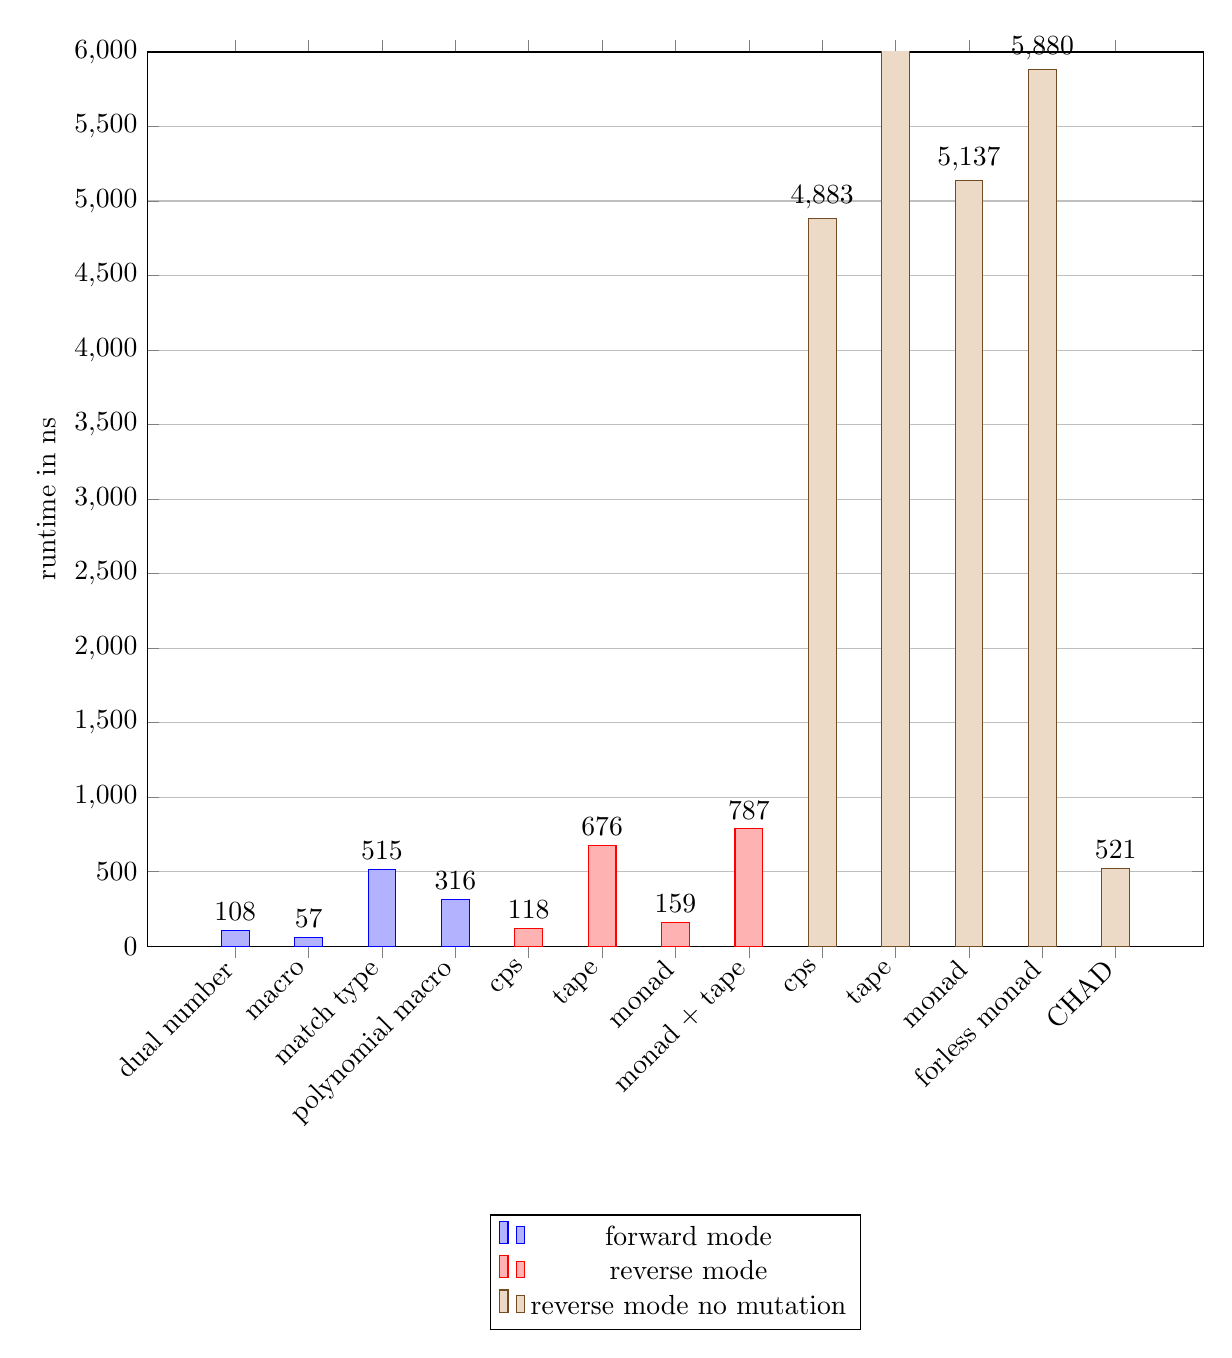
\begin{tikzpicture}%[trim axis left]
        \begin{axis}
            [
            %scale only axis,
%                symbolic x coords={dual number,dual number macro,forward match type,forward polynomial macro,reverse cps,reverse cps functional,reverse tape,reverse tape functional,reverse monad functional,reverse monad functional forless,reverse chad},
%                xtick=data,
            x tick label style={rotate=45, anchor=east, align=right},
            xtick={1,2,3,4,5,6,7,8,9,10,11,12,13},
            xticklabels={
                dual number,
                macro,
                match type,
                polynomial macro,
                cps,
                tape,
                monad,
                monad + tape,
                cps,
                tape,
                monad,
                forless monad,
                CHAD},
%                axis lines*=left,
            width=15cm,
            ymajorgrids = true,
            legend style={at={(0.5,-0.30)},anchor=north},
            ymin=0,
            ymax=6000,
            ylabel={runtime in ns},
%                bar width=5mm,
            ybar,
%                ybar interval=0.7,
%                enlarge x limits={abs=0.6cm},
            nodes near coords,
            every node near coord/.append style={color=black},
            every axis plot/.append style={
                ybar,
%                    bar width=.2,
                bar shift=0pt,
%                    fill
            }
            ]
            \addplot
            coordinates {
                (1,108)
                (2,57)
                (3,515)
                (4,316)
            };
            \addplot
            coordinates {
                (5,118)
                (6,676)
                (7,159)
                (8,787)
            };
            \addplot
            coordinates {
                (9,4883)
                (10,18856)
                (11,5137)
                (12,5880)
                (13,521)
            };


%                coordinates {(reverse cps,78) (reverse cps functional,1072) (reverse tape,192) (reverse tape functional,3818) (reverse monad functional,1029) (reverse monad functional forless,1042) (reverse chad,230)};
            \legend{forward mode,reverse mode,reverse mode no mutation}
        \end{axis}
    \end{tikzpicture}
\end{center}

\begin{center}
    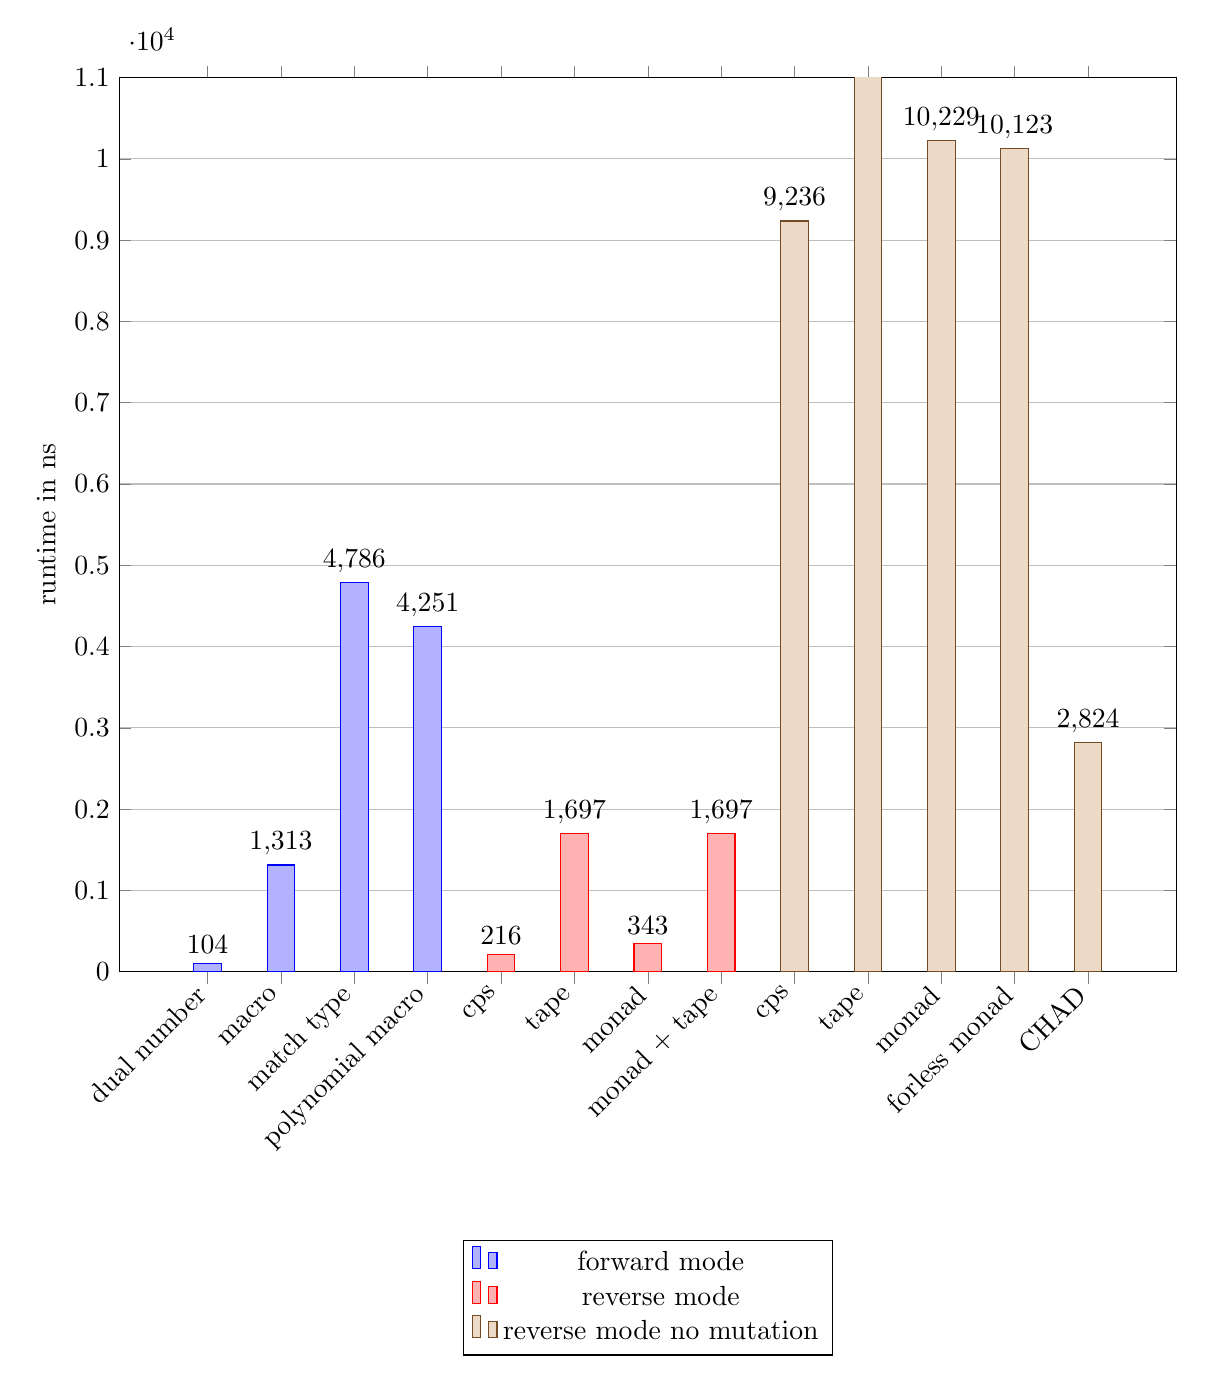
\begin{tikzpicture}%[trim axis left]
        \begin{axis}
            [
            %scale only axis,
%                symbolic x coords={dual number,dual number macro,forward match type,forward polynomial macro,reverse cps,reverse cps functional,reverse tape,reverse tape functional,reverse monad functional,reverse monad functional forless,reverse chad},
%                xtick=data,
            x tick label style={rotate=45, anchor=east, align=right},
            xtick={1,2,3,4,5,6,7,8,9,10,11,12,13},
            xticklabels={
                dual number,
                macro,
                match type,
                polynomial macro,
                cps,
                tape,
                monad,
                monad + tape,
                cps,
                tape,
                monad,
                forless monad,
                CHAD},
%                axis lines*=left,
            width=15cm,
            ymajorgrids = true,
            legend style={at={(0.5,-0.30)},anchor=north},
            ymin=0,
            ymax=11000,
            ylabel={runtime in ns},
%                bar width=5mm,
            ybar,
%                ybar interval=0.7,
%                enlarge x limits={abs=0.6cm},
            nodes near coords,
            every node near coord/.append style={color=black},
            every axis plot/.append style={
                ybar,
%                    bar width=.2,
                bar shift=0pt,
%                    fill
            }
            ]
            \addplot
            coordinates {
                (1,104)
                (2,1313)
                (3,4786)
                (4,4251)
            };
            \addplot
            coordinates {
                (5,216)
                (6,1697)
                (7,343)
                (8,1697)
            };
            \addplot
            coordinates {
                (9,9236)
                (10,69325)
                (11,10229)
                (12,10123)
                (13,2824)
            };


%                coordinates {(reverse cps,78) (reverse cps functional,1072) (reverse tape,192) (reverse tape functional,3818) (reverse monad functional,1029) (reverse monad functional forless,1042) (reverse chad,230)};
            \legend{forward mode,reverse mode,reverse mode no mutation}
        \end{axis}
    \end{tikzpicture}
\end{center}

\begin{center}
    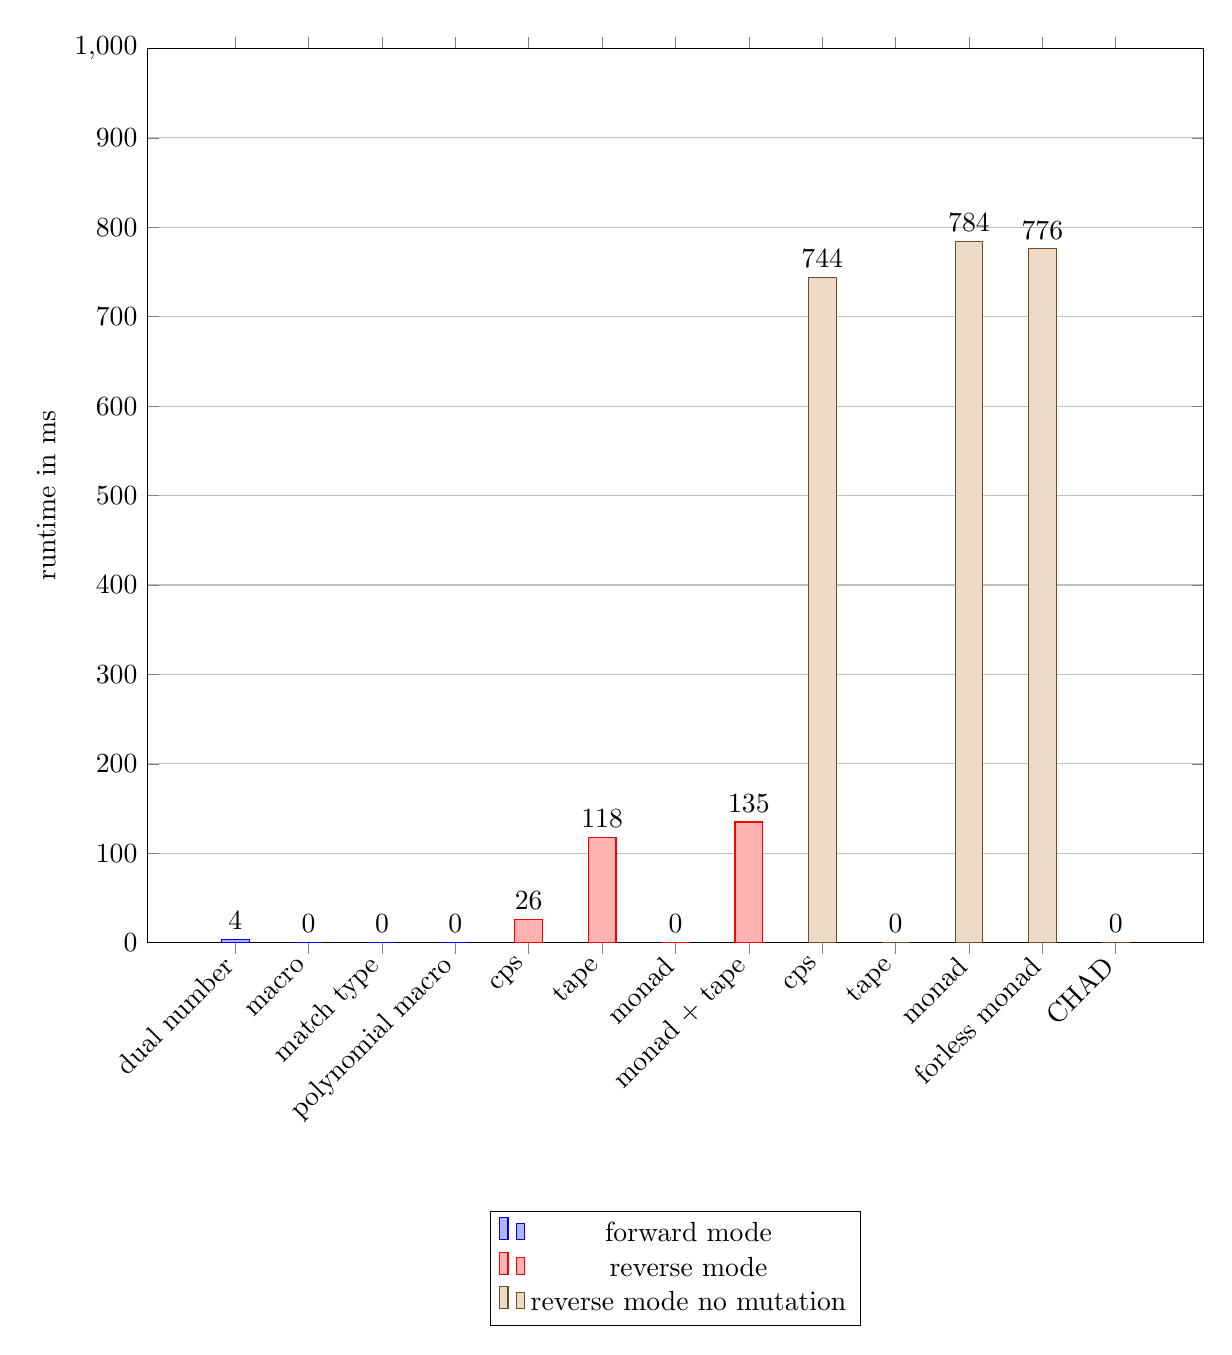
\begin{tikzpicture}%[trim axis left]
        \begin{axis}
            [
            %scale only axis,
%                symbolic x coords={dual number,dual number macro,forward match type,forward polynomial macro,reverse cps,reverse cps functional,reverse tape,reverse tape functional,reverse monad functional,reverse monad functional forless,reverse chad},
%                xtick=data,
            x tick label style={rotate=45, anchor=east, align=right},
            xtick={1,2,3,4,5,6,7,8,9,10,11,12,13},
            xticklabels={
                dual number,
                macro,
                match type,
                polynomial macro,
                cps,
                tape,
                monad,
                monad + tape,
                cps,
                tape,
                monad,
                forless monad,
                CHAD},
%                axis lines*=left,
            width=15cm,
            ymajorgrids = true,
            legend style={at={(0.5,-0.30)},anchor=north},
            ymin=0,
            ymax=1000,
            ylabel={runtime in ms},
%                bar width=5mm,
            ybar,
%                ybar interval=0.7,
%                enlarge x limits={abs=0.6cm},
            nodes near coords,
            every node near coord/.append style={color=black},
            every axis plot/.append style={
                ybar,
%                    bar width=.2,
                bar shift=0pt,
%                    fill
            }
            ]
            \addplot
            coordinates {
                (1,4)
                (2,0)
                (3,0)
                (4,0)
            };
            \addplot
            coordinates {
                (5,26)
                (6,118)
                (7,0)
                (8,135)
            };
            \addplot
            coordinates {
                (9,744)
                (10,0)
                (11,784)
                (12,776)
                (13,0) % 1625580 ns (4 nestings)
            };


%                coordinates {(reverse cps,78) (reverse cps functional,1072) (reverse tape,192) (reverse tape functional,3818) (reverse monad functional,1029) (reverse monad functional forless,1042) (reverse chad,230)};
            \legend{forward mode,reverse mode,reverse mode no mutation}
        \end{axis}
    \end{tikzpicture}
\end{center}